\documentclass[11pt,a4paper]{article}
\usepackage[utf8x]{inputenc}
\usepackage[T1]{fontenc}
%\usepackage{gentium}
\usepackage{mathptmx} % Use Times Font

\usepackage{float}
\usepackage[printwatermark]{xwatermark}
\usepackage{xcolor}
\usepackage{graphicx}
\usepackage{breakcites}
\usepackage{verbatim}
\usepackage{graphicx} % Required for including pictures
\usepackage{hyperref} % Format links for pdf
\usepackage[british]{babel} % Multilingual bibliographies
\usepackage{natbib}
\setlength{\bibsep}{0.0pt}
\setlength{\parskip}{1em}
\setlength{\parindent}{0em}

\frenchspacing % No double spacing between sentences
\usepackage[margin=1in]{geometry}

\usepackage[all]{nowidow} % Tries to remove widows
\usepackage[protrusion=true,expansion=true]{microtype} % Improves typography, load after fontpackage is selected

\usepackage{lipsum} % Used for inserting dummy 'Lorem ipsum' text into the template

\title{Edinburgh Cycle Hire in the pandemic}
\author{Karman Singh and Viren Sirwani Mulani}
%\usepackage{natbib}

\begin{document}

\maketitle

%% INSTRUCTIONS:
%%
%% 1. Please rename this file fds-project-option-1.tex,
%% fds-project-option-2.tex, or fds-project-option-3.tex, depending on
%% which project option you are doing. When you submit, please submit
%% the PDF file with the corresponding name.
%% 
%% 2. You can edit either using:
%%
%%    a. Overleaf professional, a collaborative LaTeX editor. See
%%       https://www.overleaf.com/edu/Edinburgh for documentation. Create an
%%       empty document, and copy the files in this directory to it.
%%
%%    b. A LaTeX editor on your PC - you can commit changes to this
%%       repository to collaborate.
%% 
%% 3. Please keep the section and paragraph headings as they are.
%%
%% 4. The word limit for the Overview section is mandatory. For the
%% other sections word limits are suggested.
%%
%% 5. The page limits must be strictly adhered to, and depend on if
%% you are working individually, in pairs or in threes:
%%
%%   - Individual: 6 pages 
%%   - Pairs: 8 pages 
%%   - Threes: 10 pages 
%%

\section{Overview}
% 250 words maximum
\vspace{-5mm}
The aim of this project was to understand/visualize the effect of the COVID-19 pandemic on bicycle usage in Edinburgh. We will be looking specifically at the impact of city wide lockdowns on the usage of bicycles set up by the "Just Eat" cycle scheme. The data is collected on a daily basis starting in September 2018. Comparisons were made between pre and post-lockdown with any significant changes being either visualized or scrutinized through thorough testing. We looked at various aspects of the aforementioned comparison, including the change in the popularity/usage of stations in the city. The more important question that we wanted answered was the difference in weekly usage of bikes per hour in Edinburgh. Certain restrictions were set in place by the Scottish Government, and said restrictions were speculated to have an effect on the time of the day citizens of the city would ride the bikes, be it early morning to commute to work or evening rides for leisure. We also conducted hypothesis tests on average number and duration of trips for pre-lockdown and post-lockdown months. This was to confirm our initial hypothesis of no change. The results of the above mentioned experiments were as expected. There was definite change in the popularity of stations as well as usage patterns. Many stations had seen a significant drop in use due to measures set by the government. Bike usage over the course of the day had also shifted with more people using bikes for leisure (evening use). However, one unexpected result was the rise in overall popularity over the three years covered by the data. 
\par
\textbf{Contribution}  Viren performed the data scraping of the csv files from the 'Just Eat Cycles website' and generated the map-plots concerning the popularity of stations before and after lockdown. He was in charge of the aforementioned segment in 'Exploration and analysis', 'Overview', 'Introduction' and the 'Discussion and conclusions' section. Karman was in charge of data wrangling (data cleaning, merging, etc...), Hypothesis testing and 'Average number of trips' bar charts. He wrote the 'Data description', 'Data processing' segments in the 'Data' section and also  wrote the majority of the 'Exploration and analysis' section excluding 'Station Popularity'.

\section{Introduction}
% Suggested 400 words
\vspace{-5mm}
\paragraph{Context and motivation}

%What is the area of this data science study, and why is it interesting to investigate?
Symptoms of the novel SARS-CoV-2 virus were first reported by the Wuhan Municipal Health Commission in the city of Wuhan, Hubei Province, China on the 31\textsuperscript{st} of December 2019 \cite{who_wuhan}. As of the 5\textsuperscript{th} of April 2021, 131 million cases have been reported since the initial cluster of cases in Wuhan. The Scottish Government reported the first confirmed case in the country on the 1\textsuperscript{st} of March 2020, the patient being from the Tayside area near Dundee \cite{tayside}. The study focuses on the impact of the COVID-19 pandemic on bike sharing, specifically the Just Eat Cycles scheme in the city of Edinburgh. Our work includes Data Mining, Statistical Analysis, Data Visualization and Presentation of changes in bike usage. We have focused primarily on the comparison of bike sharing before and after nationwide lock-. The lockdowns/restrictions in question are \cite{timeline}:
\begin{itemize}
    \item 23\textsuperscript{rd} March - UK lockdown (1\textsuperscript{st} lockdown)
    \item 29\textsuperscript{th} May to 21\textsuperscript{st} September - easing of restrictions
    \item 22\textsuperscript{nd} September - Scottish Government announce new restrictions on household visits and a national curfew for pubs, bars and restaurants (2\textsuperscript{nd} lockdown)
\end{itemize}
Three types of analysis have been conducted in this study: Descriptive Analysis, Exploratory Analysis (EDA) and Inferential Analysis. The study was chosen as it is related to a current and very much significant issue. People might have started cycling for leisure or the usage of these cycles might have seen a drop due to hygiene concerns. These are doubts/questions that have been answered through data analysis and have made this experience ever more interesting.
\vspace{-4mm}
\paragraph{Previous work}
 %Brief description of any previous work in this area (e.g., in the media, or scientific literature or blogs).
%E.g. Recent surveys show that most students prefer final projects to final exams \cite{Space2021}. 
Quite a significant amount of work has taken place in this area of study. Research papers have been written about, not just on the effect of the pandemic on bike sharing but also the impact of other disasters on cycle usage. 
\par
According to the 2008 study on the impact of the 7\textsuperscript{th} of July bombings in London on transport usage \cite{london_bombing}, there was an increase in "pedal cycles" and " 2-wheeled  motor  vehicles" with decreased usage of taxis and cars. Since the London Underground and the city buses were targeted by the terrorists involved, these modes of transportation were avoided the most by the citizens of London.
\par
Others have focused more on the current situation with the general consensus being that bike sharing is seen in a more favourable light, with people preferring cycling over other modes of transportation. In Thessaloniki, Greece, bike sharing has become a more attractive "mobility option" \cite{greece_covid}, with the "importance of safety" towards COVID-19 being the main reason. Answers were given through a questionnaire survey, with 223 people taking part in the investigation. This is further backed by the investigation that took place in San Antonio, Texas, USA, where respondents would likely use the bike sharing system after restrictions are lifted \cite{texas_covid}. However, it must be noted that the increased reliance on the bike sharing system was by the unemployed (43\%).
\vspace{-4mm}
\paragraph{Objectives}
%What questions are you setting out to answer?
There is no one question we sought out to answer, however, the main objective in this case being the comparison of bike usage before and after lockdown. We will be looking at the effect of lockdown on the number of trips during the course of the day. We will also check if lockdown has had an impact on the duration of bike trips, which we will answer via a hypothesis test. Many areas of Edinburgh saw significant changes in the number of trips taken, some of which suffered a big drop in usage. It is was then decided we would identify these stations and visualize them on "map plots". The converse (increased usage) was not considered as many stations were opened during the pandemic, which makes this aspect of the investigation quite tricky, hence, was left out. 

\section{Data}
% Suggested 300 words
\vspace{-5mm}
\paragraph{Data provenance} 
% Who created the dataset(s)?  How you have obtained it (e.g., file or web scraping), and do the T\&Cs allow you to use obtain the data for the project?

The data is provided by the official Edinburgh cycle hire scheme, which is sponsored by the online food order and delivery service Just Eat. The Just Eat cycle data set is available on their website and is collected on a daily basis (published at midnight UTC) as people use the bikes. Data is available in two forms; JSON or CSV files. We decided to go with the latter format. There was quite a significant amount of files available, so, data was obtained through web scraping. The BeautifulSoup Python package was used to create a simple script that would scrape all CSV files and store them in a local directory. Fortunately, the data is published under the Open Government Licence (OGL) v3.0. Under this license,  users are allowed to "copy, publish, distribute, transmit ...adapt the Information". We are also allowed to exploit the information for non-commercial use, which was the intent of the project.   
\vspace*{-1cm}
\paragraph{Data description} %Description of the data, e.g. variables in each table, number of records.
\begin{center}
\begin{tabular}{ ||c|c|c|| } 
 \hline
 Variable & Format & Description\\ [0.5ex] 
 \hline \hline
 started\_at & Timestamp & Timestamp of when the trip started\\ 
 \hline
 ended\_at & Timestamp & Timestamp of when the trip ended \\ 
 \hline
 duration & Integer & Duration of trip in seconds \\ 
 \hline
 start\_station\_id & Integer & Unique ID of start station \\
 \hline
 start\_station\_name & String & Name of start station \\
 \hline
 start\_station\_description & String & Description of location of start station \\
 \hline
 start\_station\_latitude & Decimal degrees in WGS84 & Latitude of start station\\
 \hline
 start\_station\_longitude & Decimal degrees in WGS84 & Longitude of start station\\
 \hline
 end\_station\_id & Integer & Unique ID of end station\\
 \hline
 end\_station\_name & String & Name of end station\\
 \hline
end\_station\_description & String & Description of location of end station \\
\hline
end\_station\_latitude & Decimal degrees in WGS84 & Latitude of end station\\
\hline
end\_station\_longitude & Decimal degrees in WGS84 & Longitude of end station\\
 \hline
\end{tabular}
\end{center} 
%
We scraped a total of 384589 records, starting on the 15\textsuperscript{th} of September 2019 to the end of March 2021. 
\vspace{-4mm}

\paragraph{Data processing} %How you have processed the dataset, e.g., cleaning, removing missing values, joining tables.

After scraping the CSV files off of the Just Eat Cycles website, we concatenated all the files into a data-frame named "cycles". Data cleaning then took place, where rows with empty/missing values were removed from the dataset. We proceeded to add a new variable named "start\_hour" which stored the hour of the day of when the trip started. We converted the latitude and longitude values, which were given in degrees, to radians. This helped us calculate the displacement of the trip (between the start and end station) and allowed for additional analysis of the data. The dataset was initially separated into the individual year the data was collected. We further segregated the "cycles" data-frame based on whether the trip started before lockdown, during lockdown, in summers or in winters of 2019/2020.

\section{Exploration and  analysis}
% Suggested 500 words for individual report; proportionately longer
% for group projects).
\subsection{Visualizing number of Trips per Month}
\vspace{-5mm}
We commenced our analysis by plotting a line graph of the total number of bike trips per month from September 2018 to March 2021 (Figure~\ref{total_trips_per_month}) in order to examine whether there were any visible patterns that emerged.
\par
We found that the number of trips remained relatively constant until February of 2019, after which there was an overall increase in the total number of trips until August of 2019. It's possible that this is due to the success and increasing popularity of the "Just Eat Cycles" hire scheme \cite{hire_scheme} among the citizens and students living in Edinburgh. We can see a moderate decrease in the number of bike trips from August to December of 2019, which may be due to the decrease in average temperature in Edinburgh \cite{average_temp}. We observed an overall increase in the number of trips from December of 2019 to April of 2020 with a slight decrease in February of 2020 which based on our analysis was caused by a slight decline in the average temperature.
We also noticed a spike in the number of bike trips from April to May of 2020 and we conjectured that this was due to higher average temperature in May as compared to that in April. There were no drastic changes in the number of trips till August of 2020 which was near the end of the summer season. There was a gradual decrease in the number of bike trips from August 2020 to January 2021. Based on our initial speculation, this could have been due to a combination of increasing harsh weather conditions and strengthening of lockdown restrictions.

\begin{figure}[h]
    \centering
    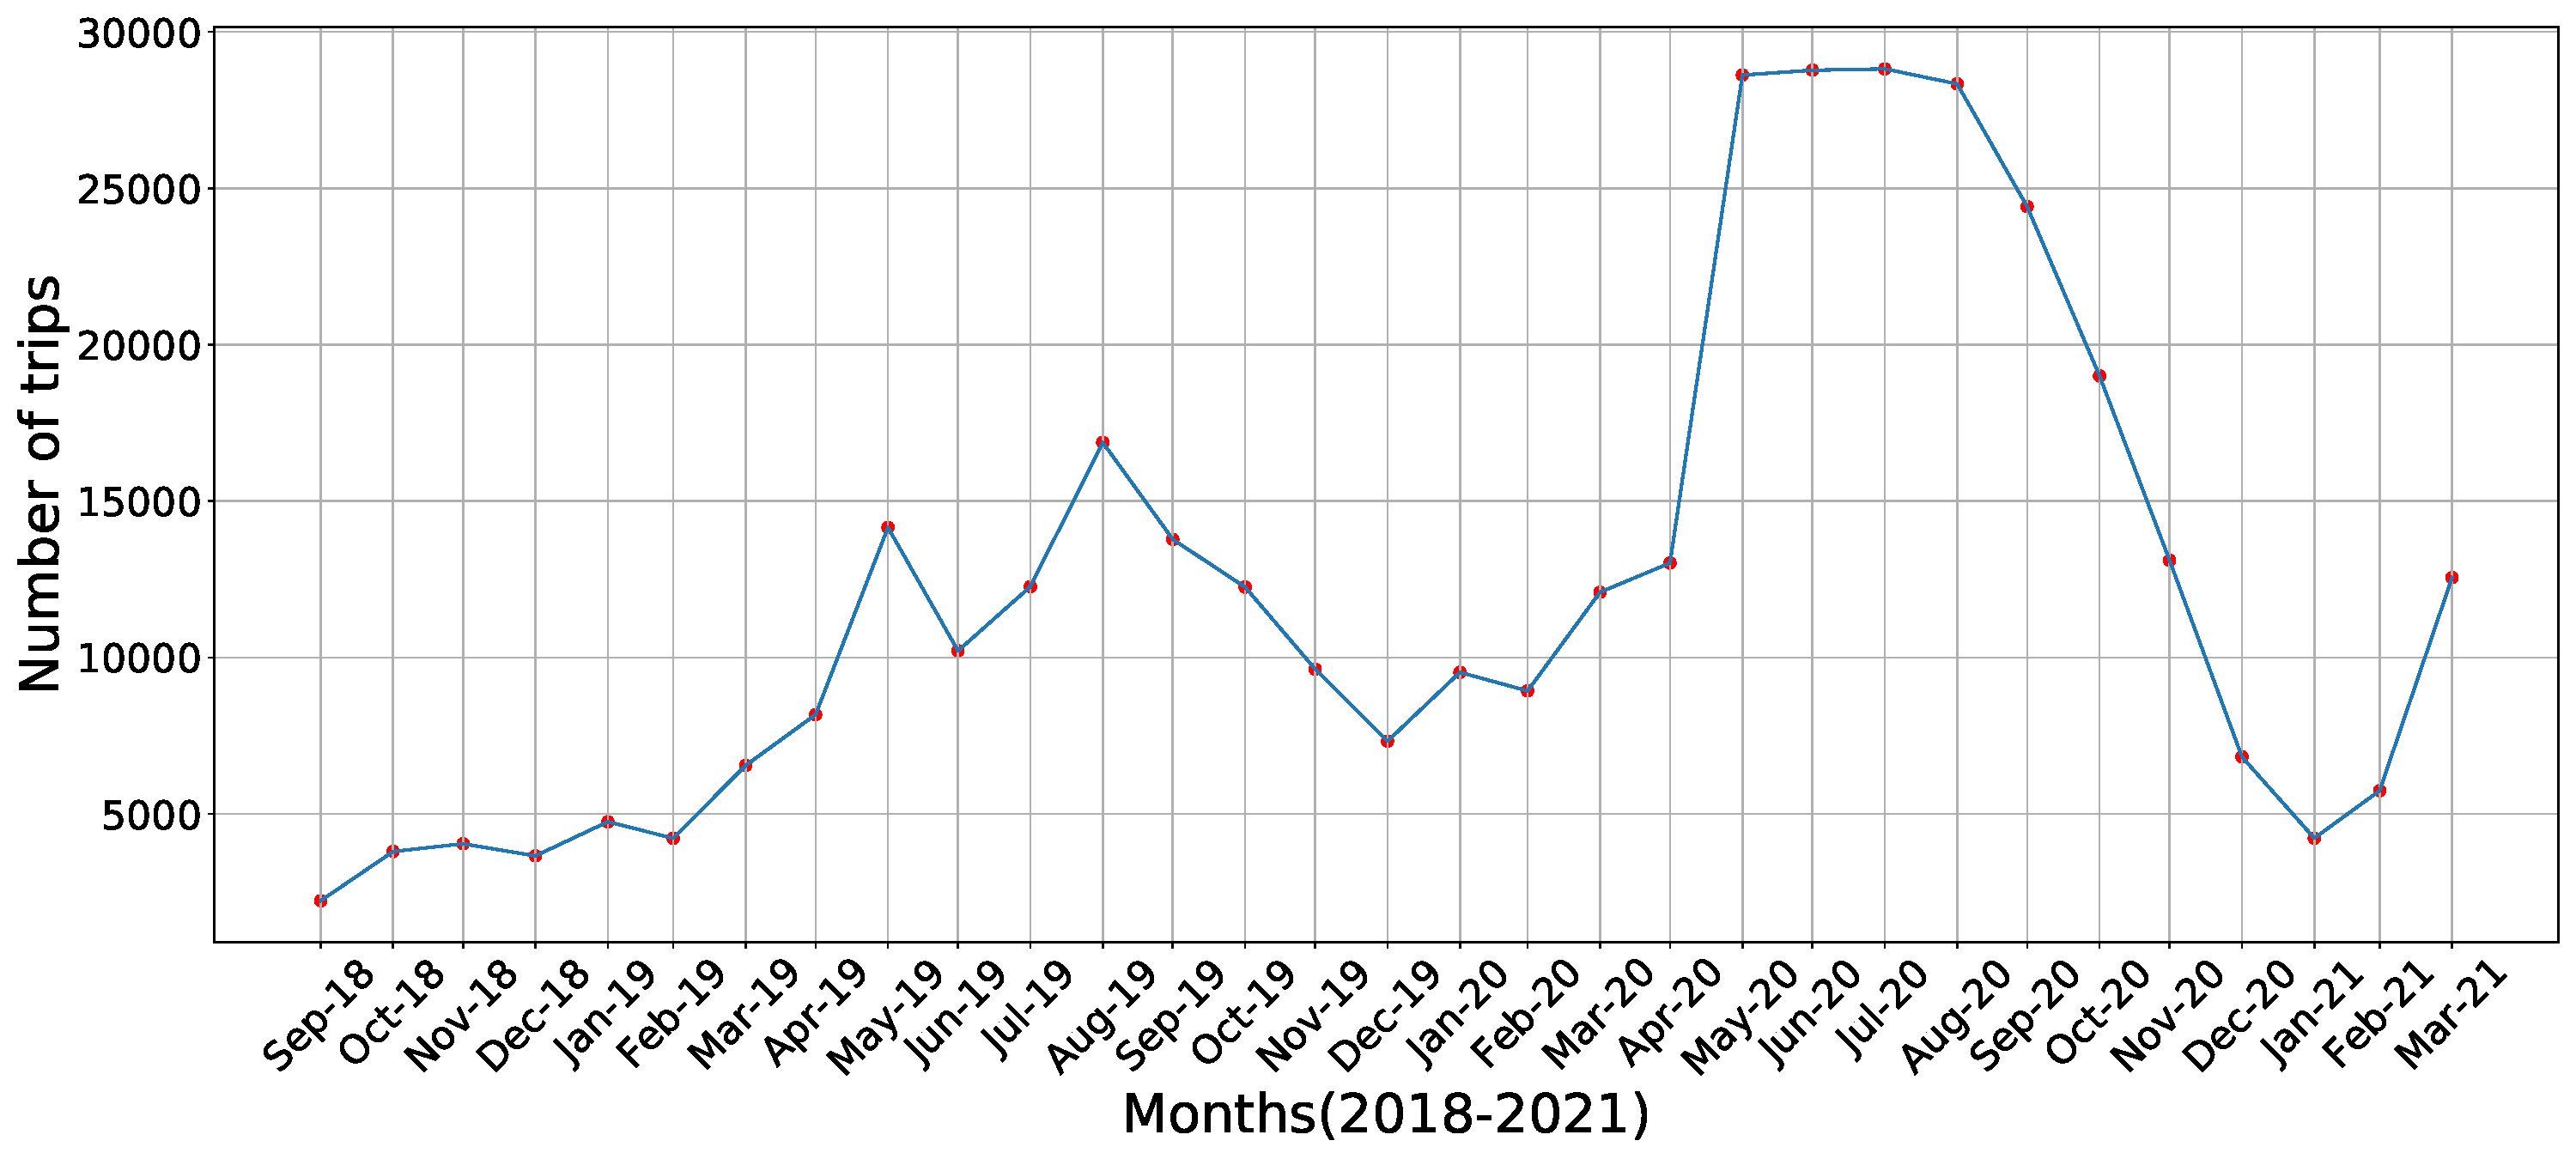
\includegraphics[width=\linewidth]{datasets/total_trips_per_month.pdf}
    \caption{Number of trips per month from September 2018 to March 2021}
    \label{total_trips_per_month}
\end{figure}

\subsection{Hypothesis Testing}
\vspace{-5mm}
We proceeded to conduct a Hypothesis test on the average duration of the bike trips during the pre-lockdown and post-lockdown period at the 5\% significance level to answer the main objective question, i.e, whether lockdown had an effect on the average bike usage in Edinburgh.
\par
The null and alternative hypothesis were as follows :
\vspace{-5mm}
\begin{itemize}
  \item \(H_{0}\) : Lockdown has no effect on the average duration of the bike trips
  \item \(H_{A}\) : Lockdown has some effect on the average duration of the bike trips
\end{itemize}
We performed a two-sample t-test on the 'duration' column of the 'pre\_lockdown' and 'post\_lockdown' dataset where the variance was unknown. The procedure was as follows :
\vspace{-5mm}
\begin{itemize}
    \item We first calculated the t-statistic, assuming the null hypothesis(\(H_0\)) was true. \vspace{1mm}\[T-Statistic, T = \frac{\bar{X}-\bar{Y}}{\sqrt{S_p^2(\frac{1}{n} + \frac{1}{m})}} \sim\ t_{n+m-2}\]
    where $\bar{X}$ is the average duration of bike trips before lockdown started, $\bar{Y}$ is the average duration of bike trips after lockdown started, n is the total number of bike trips before the \(1^{st}\) lockdown (\(23^{rd}\) March), m is the total number of bike trips after the first lockdown, \(S_p^2\) is the pooled variance of the 2 datasets.
    \item -15.1001 was the calculated t-statistic value and 1.74e-51 was the corresponding p-value. 
    \item Since the p-value is significantly smaller than the significance level of 5\%, there is enough evidence to reject the null hypothesis, i.e., lockdown has no effect on the average duration of the bike trips, in favour of the alternative hypothesis.
\end{itemize}

\subsection{Effect of Lockdown on Bike Usage}
\vspace{-5mm}
%analysis of the plot for number of trips before/during lockdown grouped by hour
We further analysed the total number of bike trips before and after the first lockdown  (Figure~\ref{total_trips_pre_post_lockdown_grouped_by_hour}) by categorising the data based on when the trip began. We noticed that the number of trips in the early hours of the day (7AM-8AM) was higher before lockdown started. This could have been caused due to the "work from home" restriction that was introduced at the start of the first lockdown which meant that most of the working mass did not need to commute to work in the early hours of the day which in turn lead to a decrease in the number of bike trips during lockdown. We also noticed that contrary to our initial speculation, the number of trips throughout the day, from 10AM to  10PM, were higher during lockdown as compared to that before lockdown. Upon further analysis we concluded that this could have been due to the growing interest in cycling and the public's preference of avoiding public transports.

\begin{figure}[h]
    \centering
    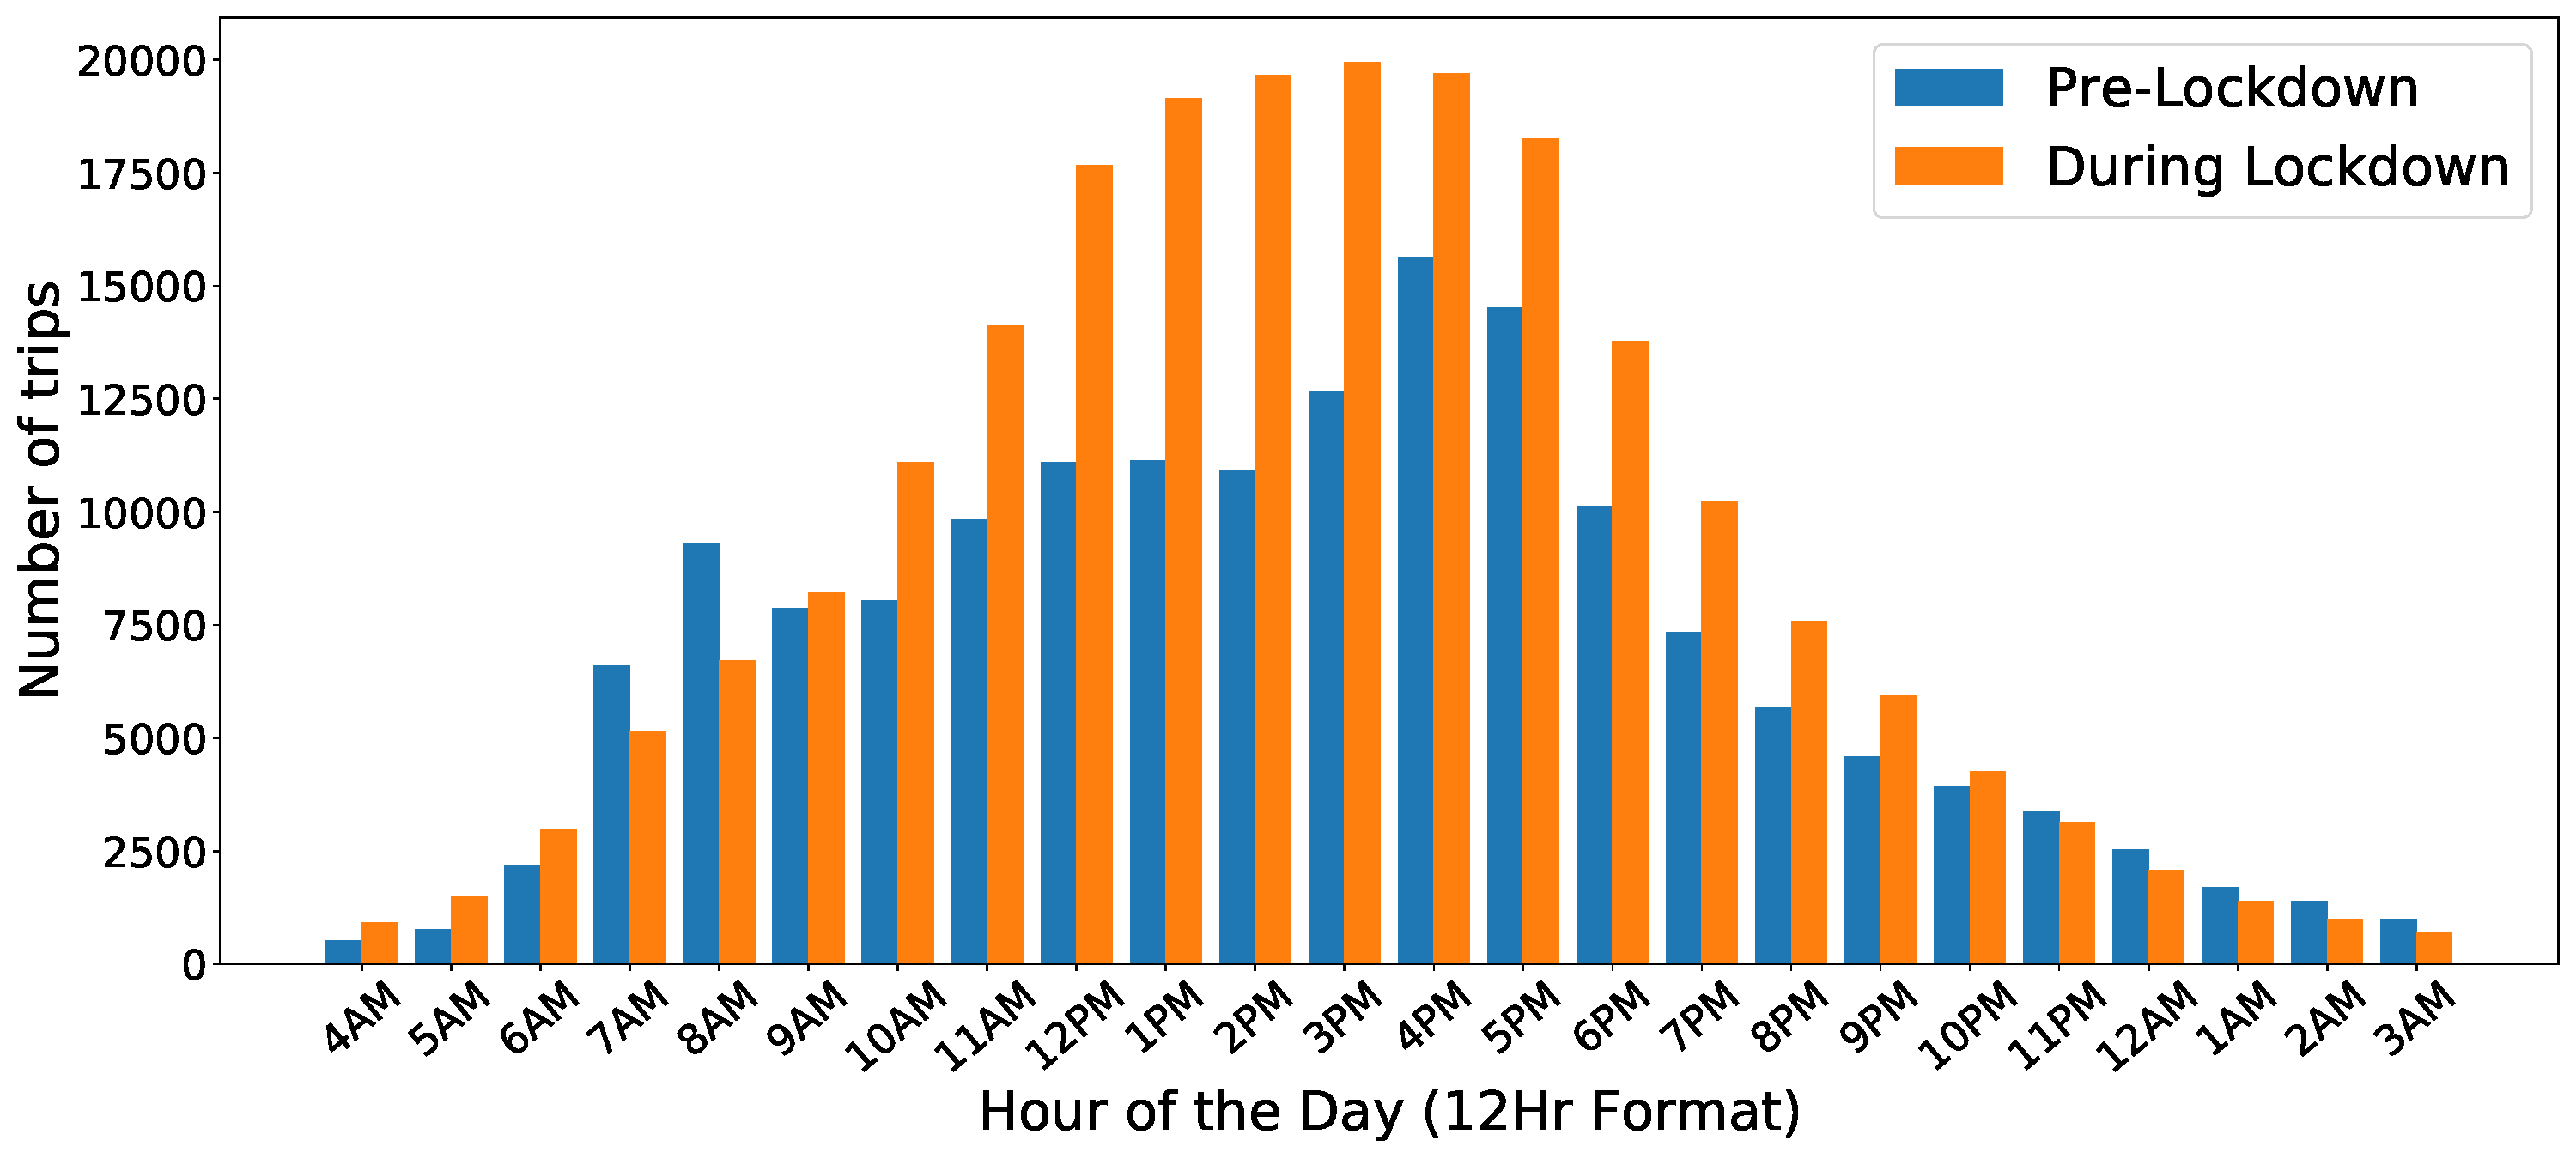
\includegraphics[width=\linewidth]{datasets/total_trips_by_hour_pre_post_lockdown.pdf}
    \caption{Number of bike trips before and during lockdown grouped by hour}
    \label{total_trips_pre_post_lockdown_grouped_by_hour}
\end{figure}

\subsection{Comparison between Seasons}
\vspace{-5mm}
In order to analyse the difference in bike usage during summers and winters of 2019 and 2020, we categorised the summers and winters dataset based on when the trip began and plotted the average number of bike trips per week during Summers and Winters of 2019 and 2020. We noticed that the average number of trips in Summers of 2020 followed a normal distribution and also the graph for Winters of 2019 was bi-modal which indicated that there were 2 distinct peaks in the number of bike hires per day.
\par
\begin{figure}[h]
    \centering
    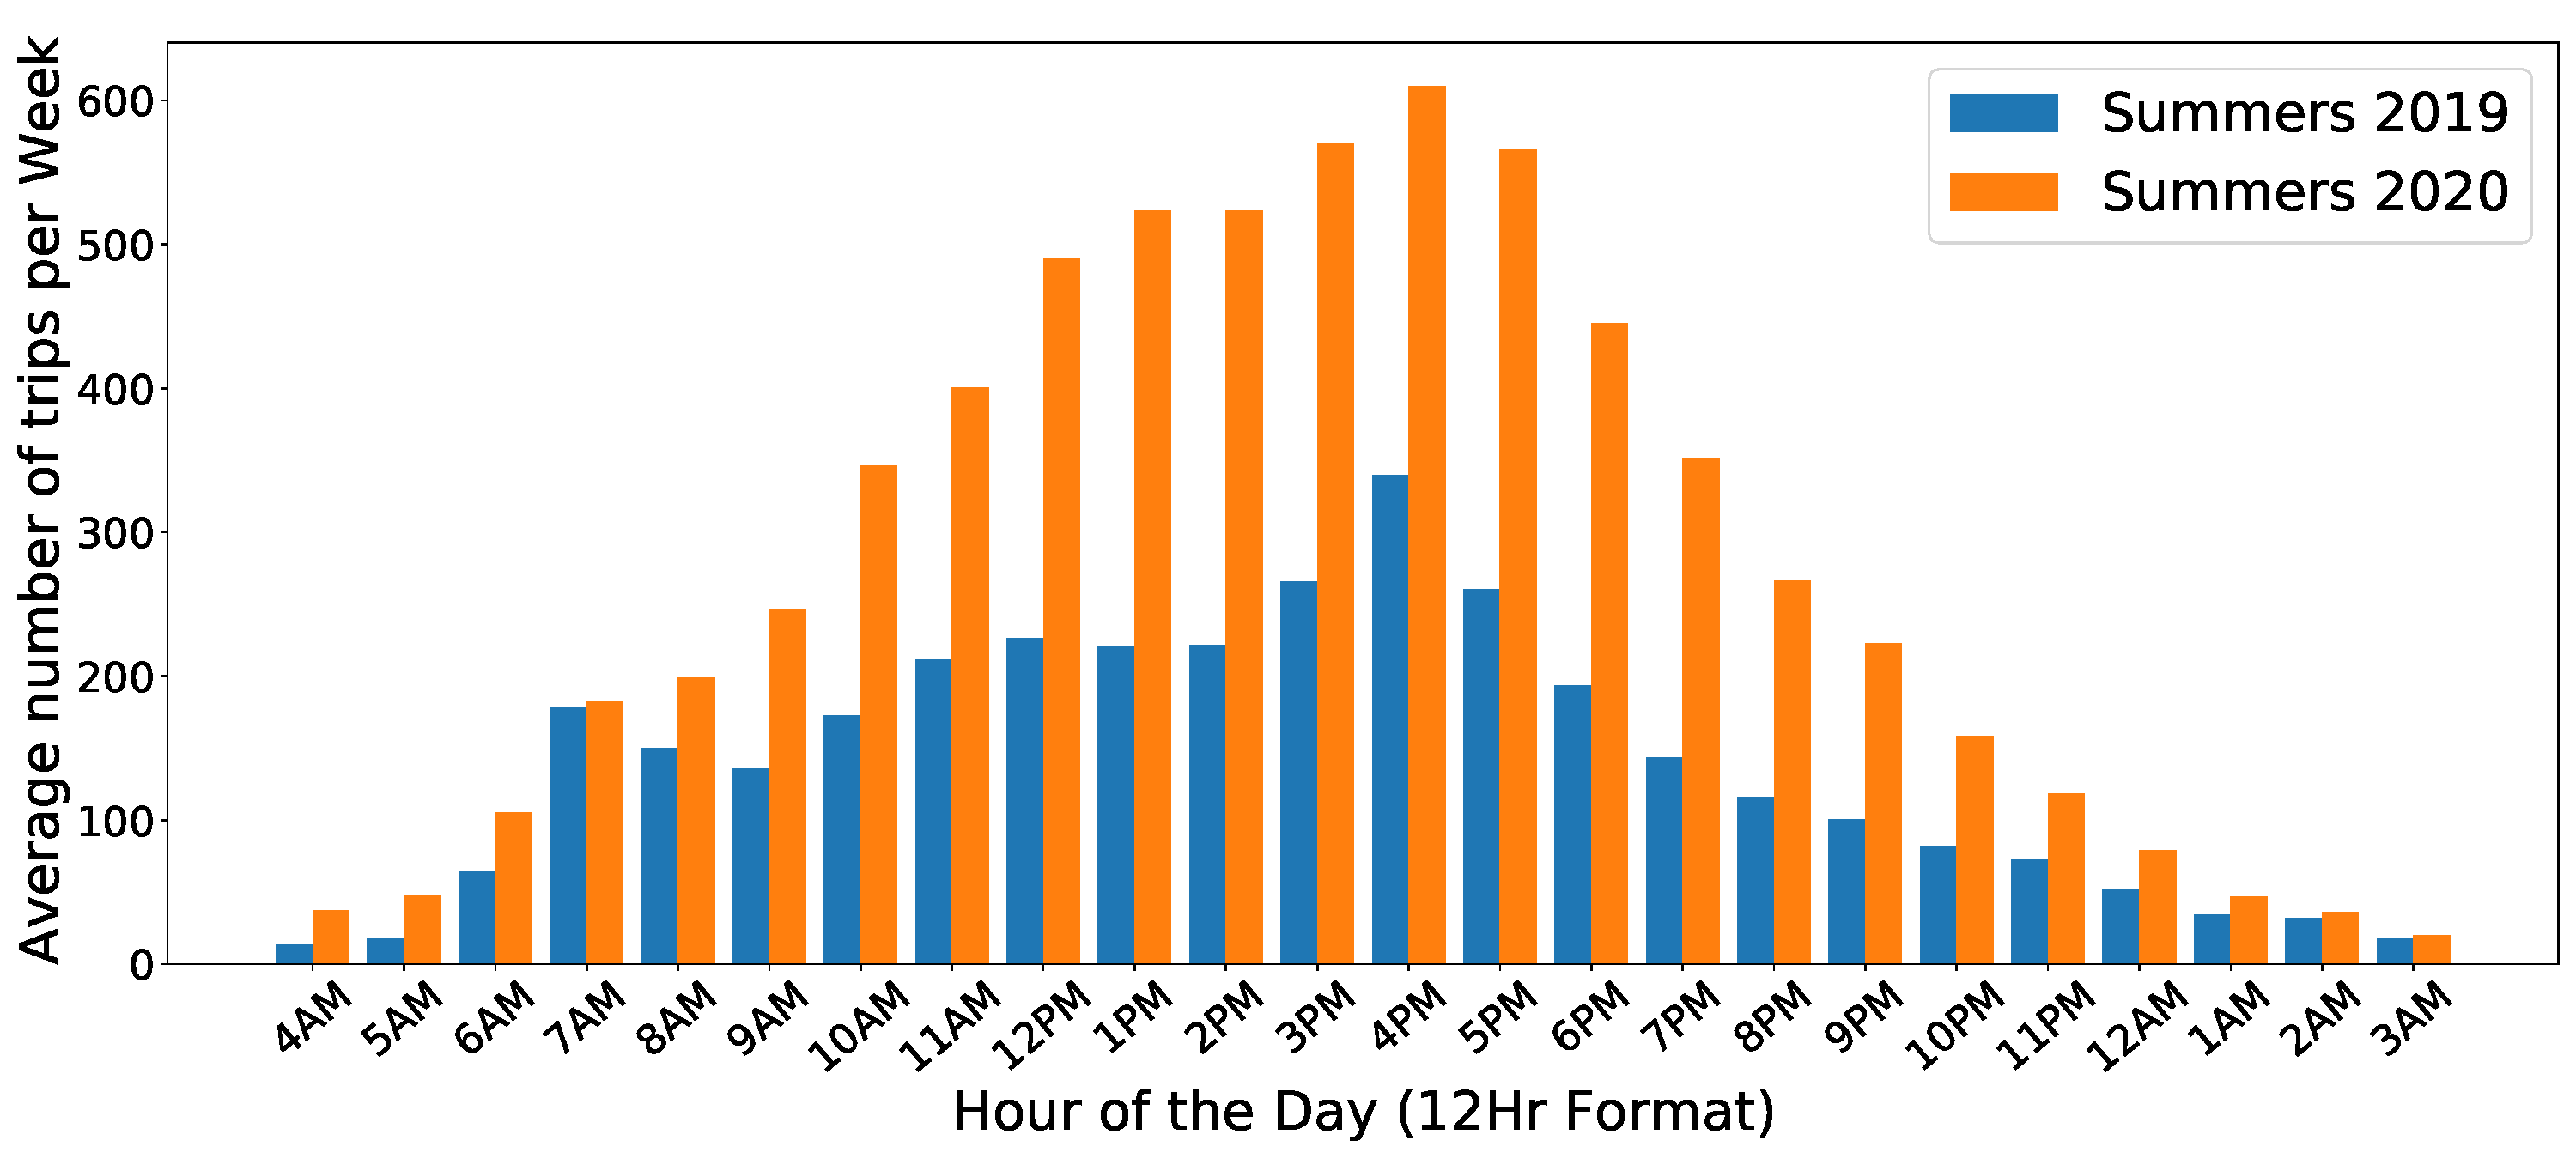
\includegraphics[width=\linewidth]{datasets/summers_weekly_bike_usage_by_hour.pdf}
    \caption{Average number of bike trips per week grouped by hour in Summers of 2019 and 2020}
    \label{average_trips_per_week_summers}
\end{figure}
In Figure~\ref{average_trips_per_week_summers}, we can clearly see that throughout the day, the average number of trips per week was lower during summers of 2019 as compared to summers of 2020. Based on our analysis, this rise in the average number of trips was due to the growing interest in cycling as an outdoor activity by the citizens and students living in Edinburgh. Due to the restrictions that were put in place caused by the rising number of SARS-CoV-2 cases, people preferred to avoid public transports like buses and taxis, and instead either just walk or use bikes. 
\par
On the other hand, in Figure~\ref{average_trips_per_week_winters}, we can see that throughout the day, the average number of trips per week was higher during Winters of 2019 as compared to Winters of 2020. We concluded that the main reasons for the drop in the average number of trips per week from 2019 Winters to 2020 Winters were due to the second lockdown restrictions that were introduced in September of 2020 and also due to the snow storms that were experienced during the winters of 2020 \cite{snow_storm}. 

\begin{figure}[h]
    \centering
    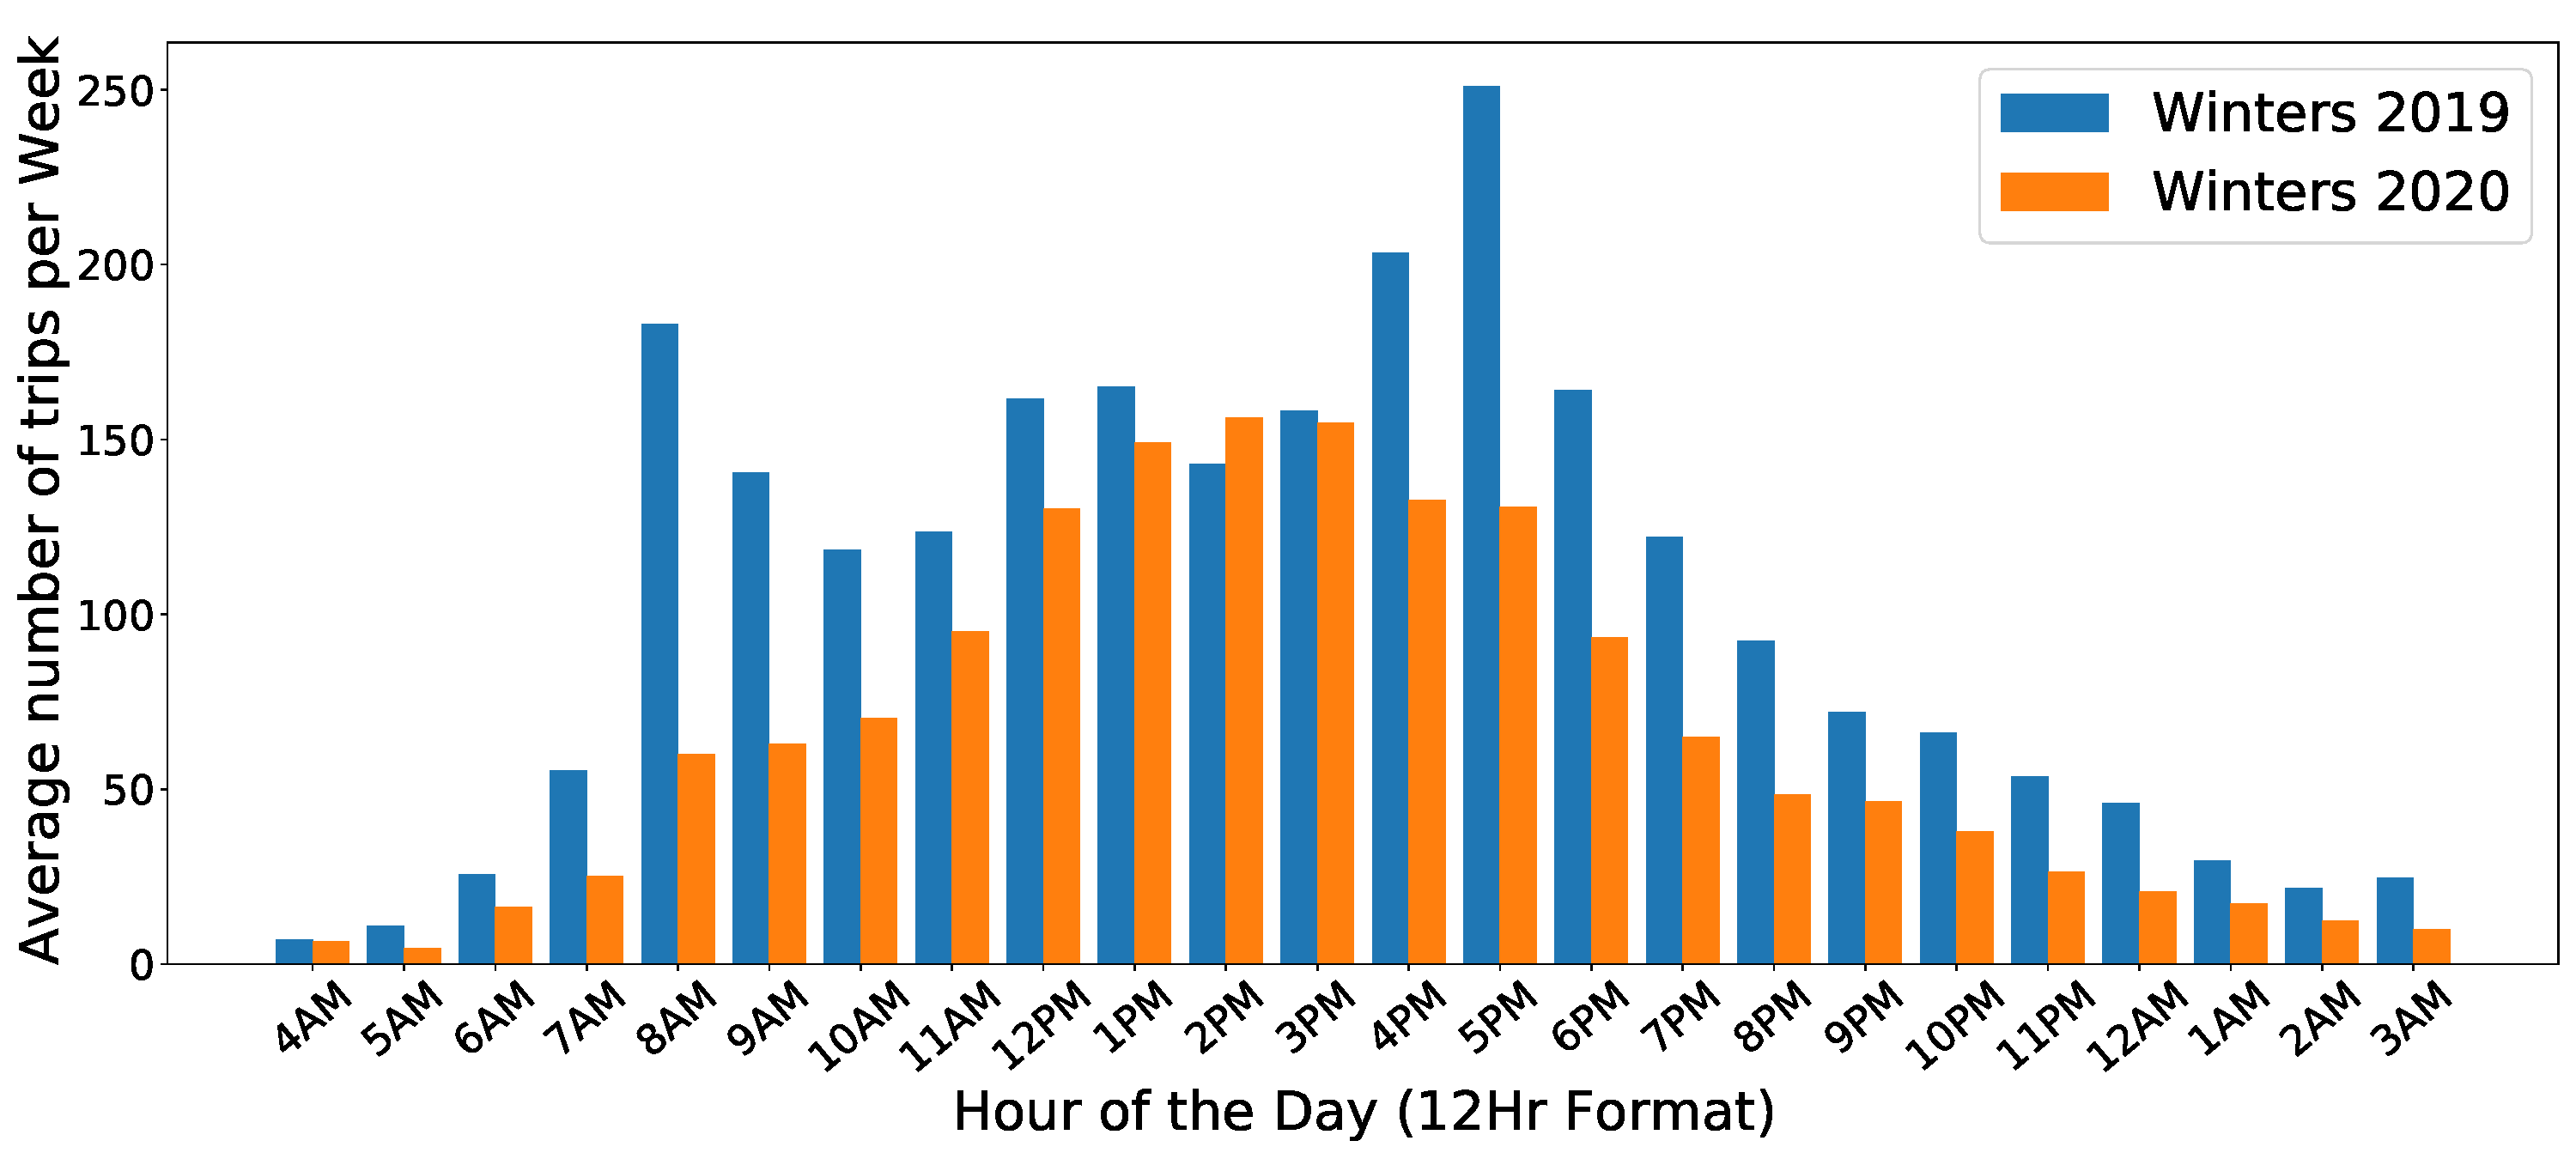
\includegraphics[width=\linewidth]{datasets/winters_weekly_bike_usage_by_hour.pdf}
    \caption{Average number of bike trips per week grouped by hour in Winters of 2019 and 2020}
    \label{average_trips_per_week_winters}
\end{figure}
%\clearpage
%analysis of popular stations and % difference
\subsection{Station Popularity}
\vspace{-5mm}
Many stations across the city had been impacted by the pandemic, which lead to changes in the usage of bikes in certain areas of Edinburgh. We first looked at the most popular stations, i.e. the stations with the most number of trips, and plotted geographic data onto a map of Edinburgh and its surroundings. The difference between Figure~\ref{pre_lockdown_popularity} and Figure~\ref{post_lockdown_popularity} is quite significant in the sense that the more popular stations are now located further north, with many found in Leith. Most popular stations were concentrated in Old Town, New Town and West End which are three densely populated areas, known for being the main commercial districts of Edinburgh. 
\par 
Due to lockdown, very few stores were open on Princess Street \cite{stores_princess}. As already mentioned, leisure became primary/most common usage of bikes after lockdown, with three popular stations located on the seafront. Stations in residential areas became more popular due to restrictions placed by the Scottish Government causing many establishments in the city to close down \cite{establishments}. The overall impact of city wide restrictions can be seen in Figure~\ref{percentage_popularity}.
\begin{figure}[h]
    \centering
    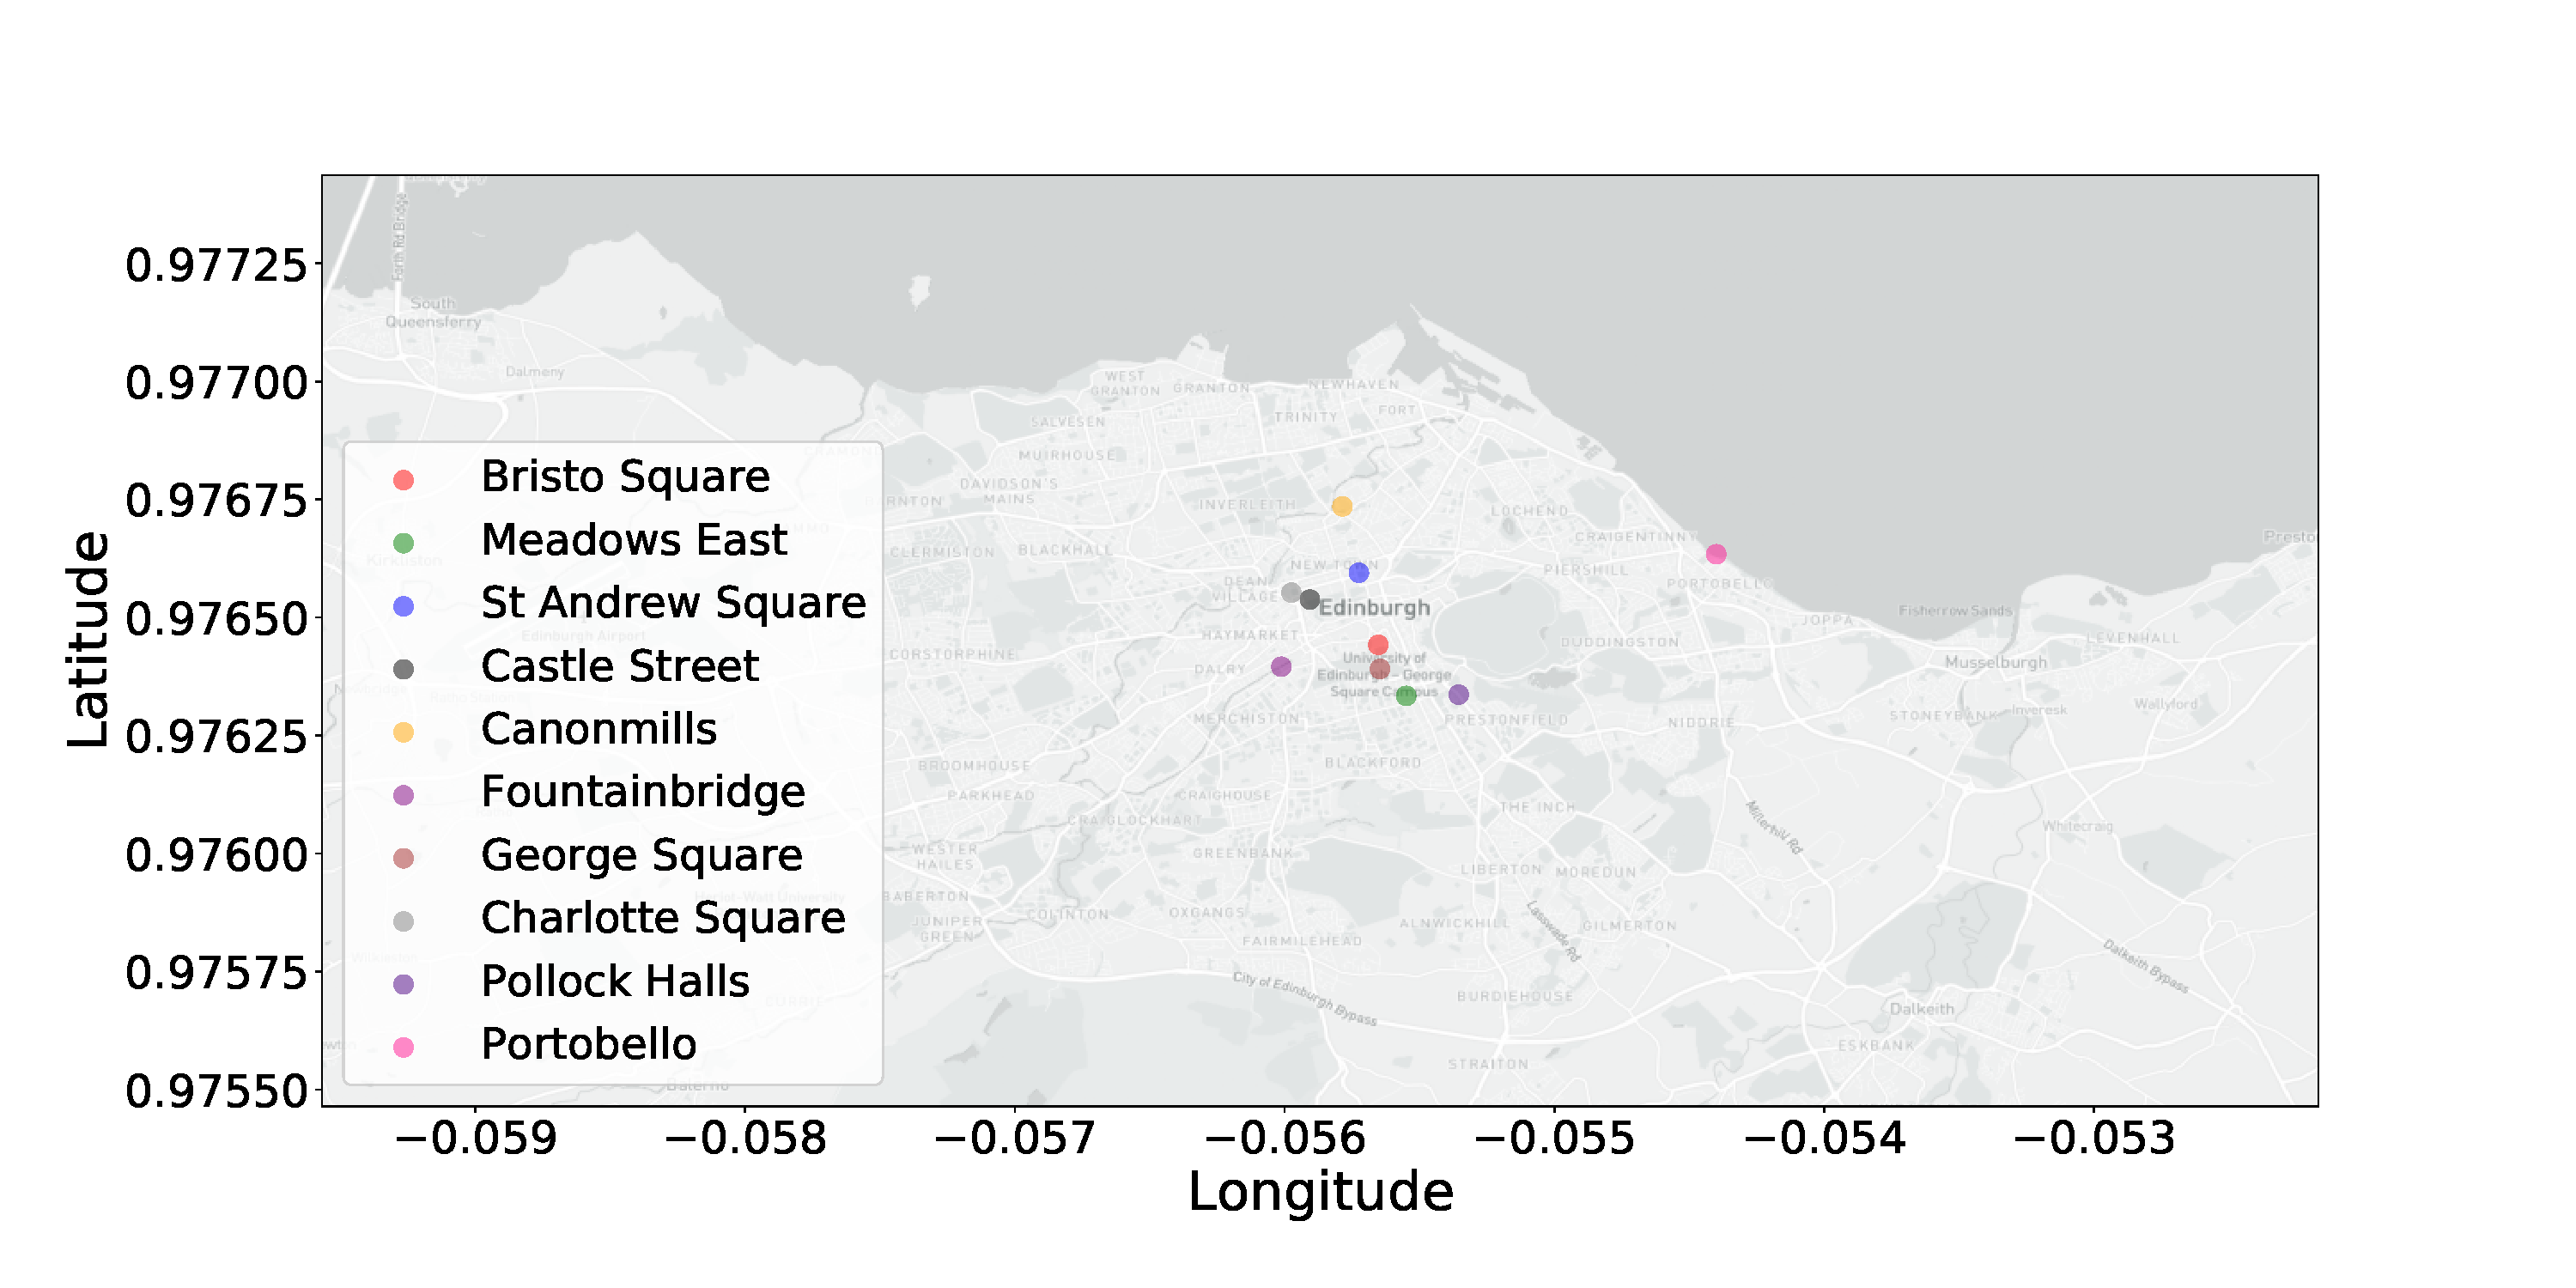
\includegraphics[width=\linewidth]{datasets/popular_stations_pre_lockdown.pdf}
    \vspace*{-1.3cm}
    \caption{Most popular stations pre-lockdown}
    \label{pre_lockdown_popularity}
\end{figure}
\vspace*{-2cm}
\begin{figure}[H]
    \centering
    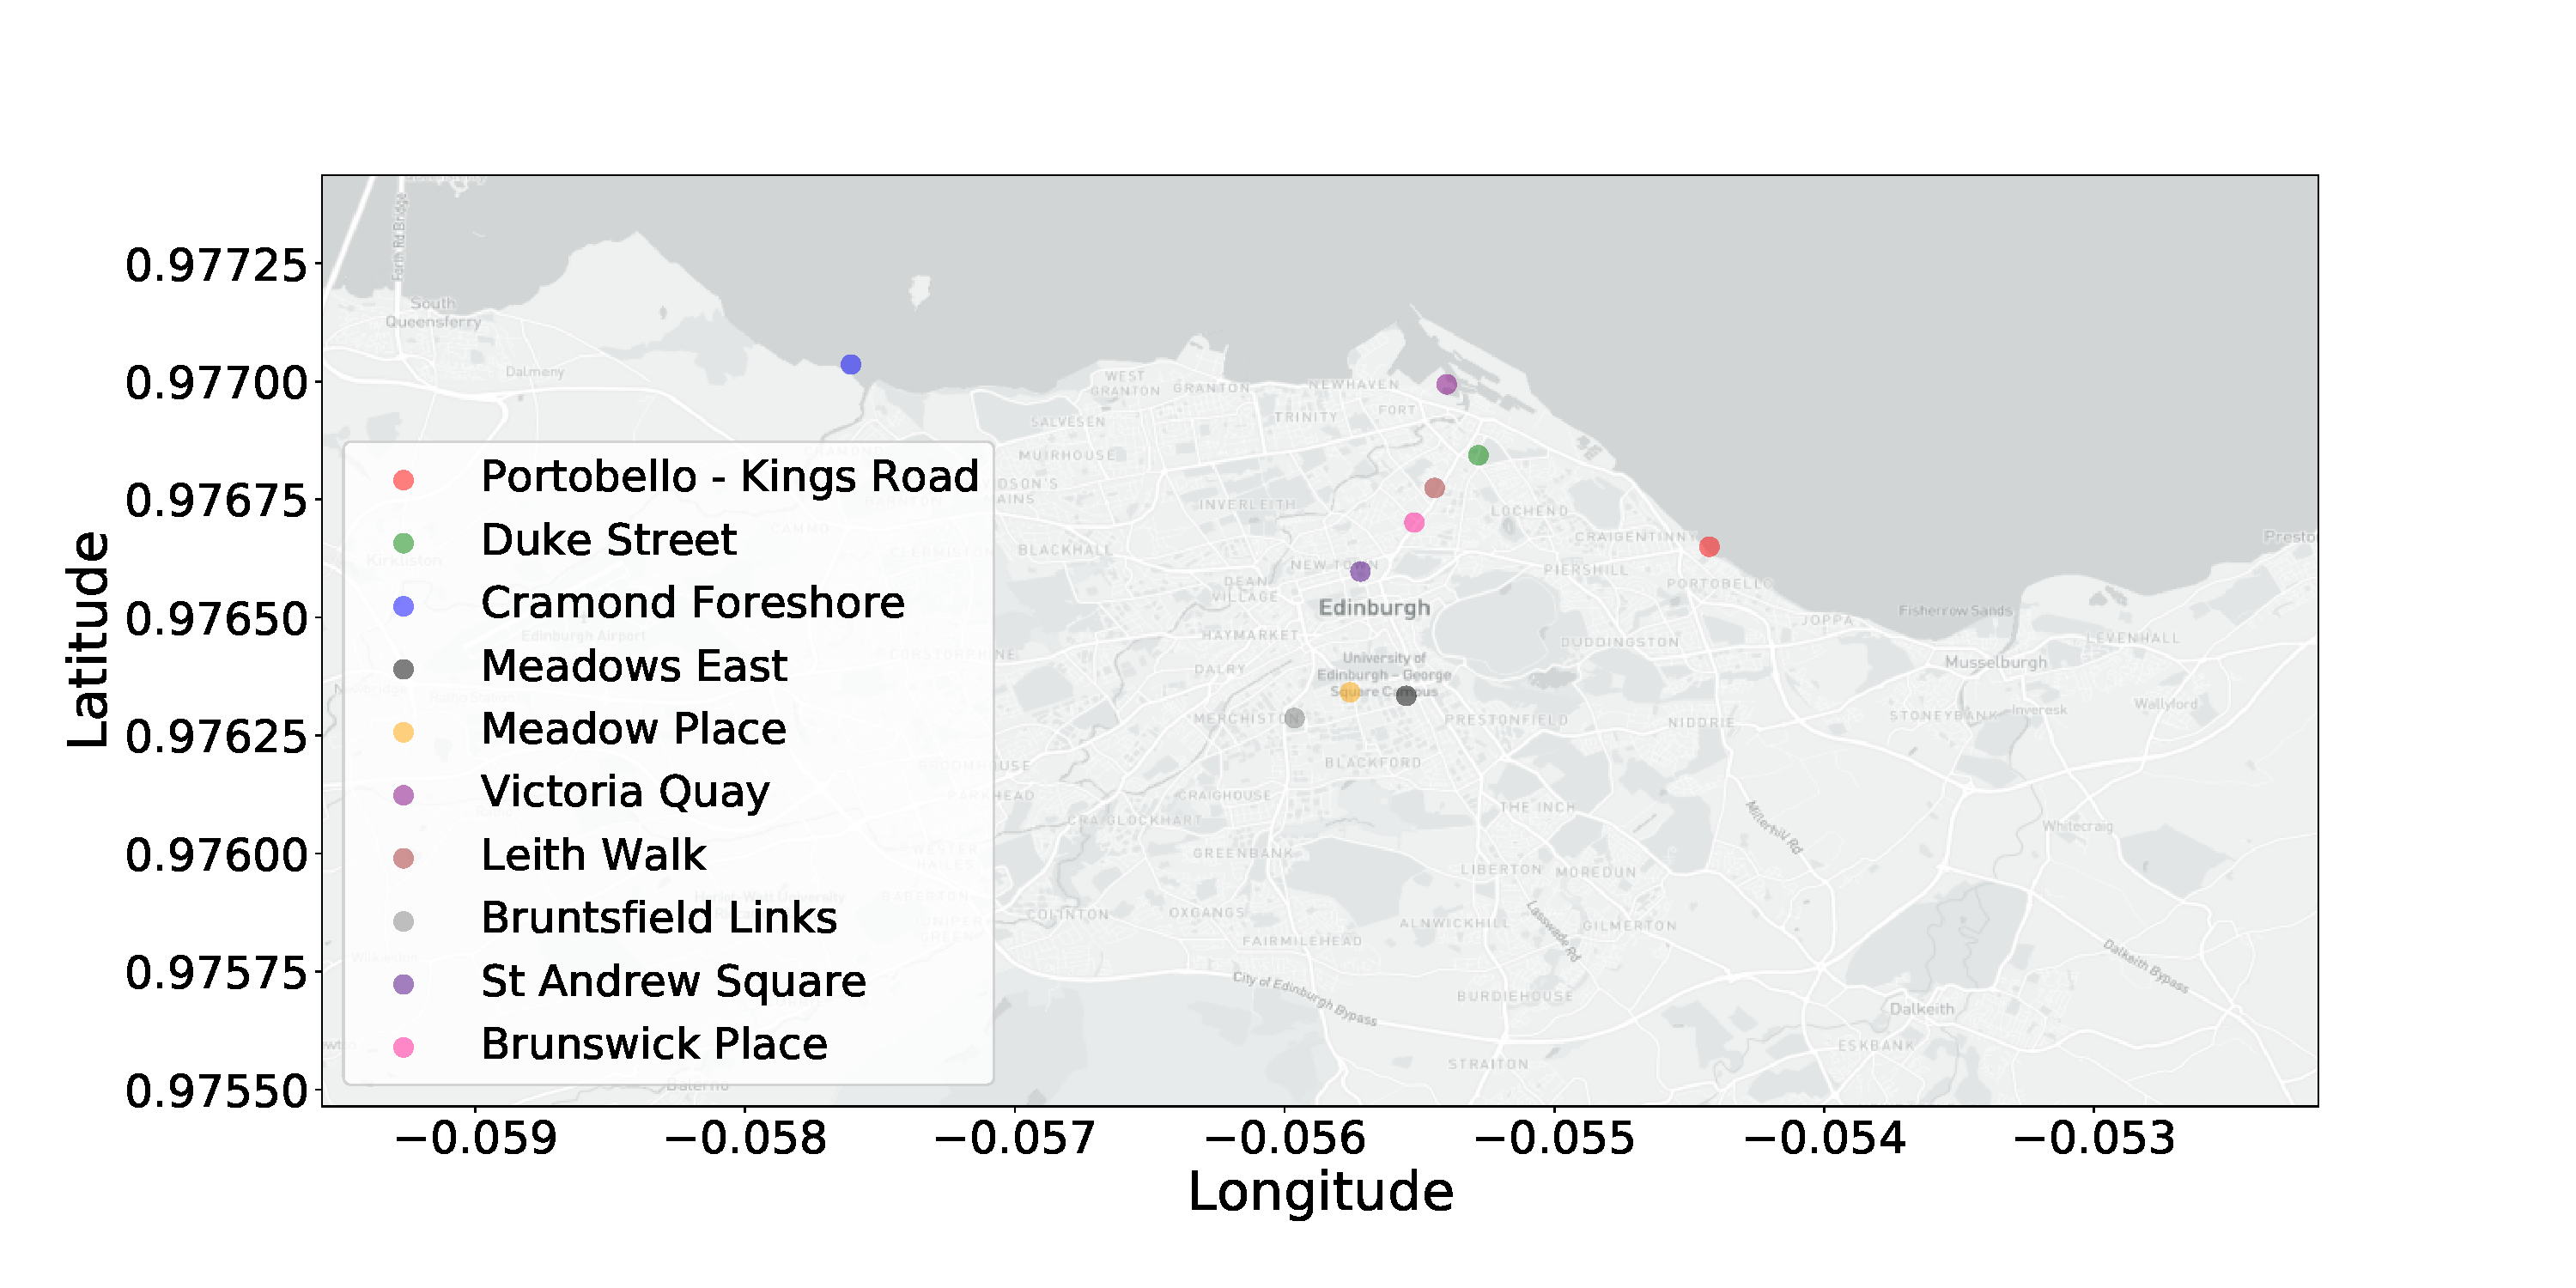
\includegraphics[width=\linewidth]{datasets/popular_stations_post_1st_lockdown.pdf}
    \vspace*{-1.3cm}
    \caption{Most popular stations post 1\textsuperscript{st} lockdown}
    \label{post_lockdown_popularity}
\end{figure}
\vspace*{-1cm}
\begin{figure}[h]
    \hspace*{-1cm}
    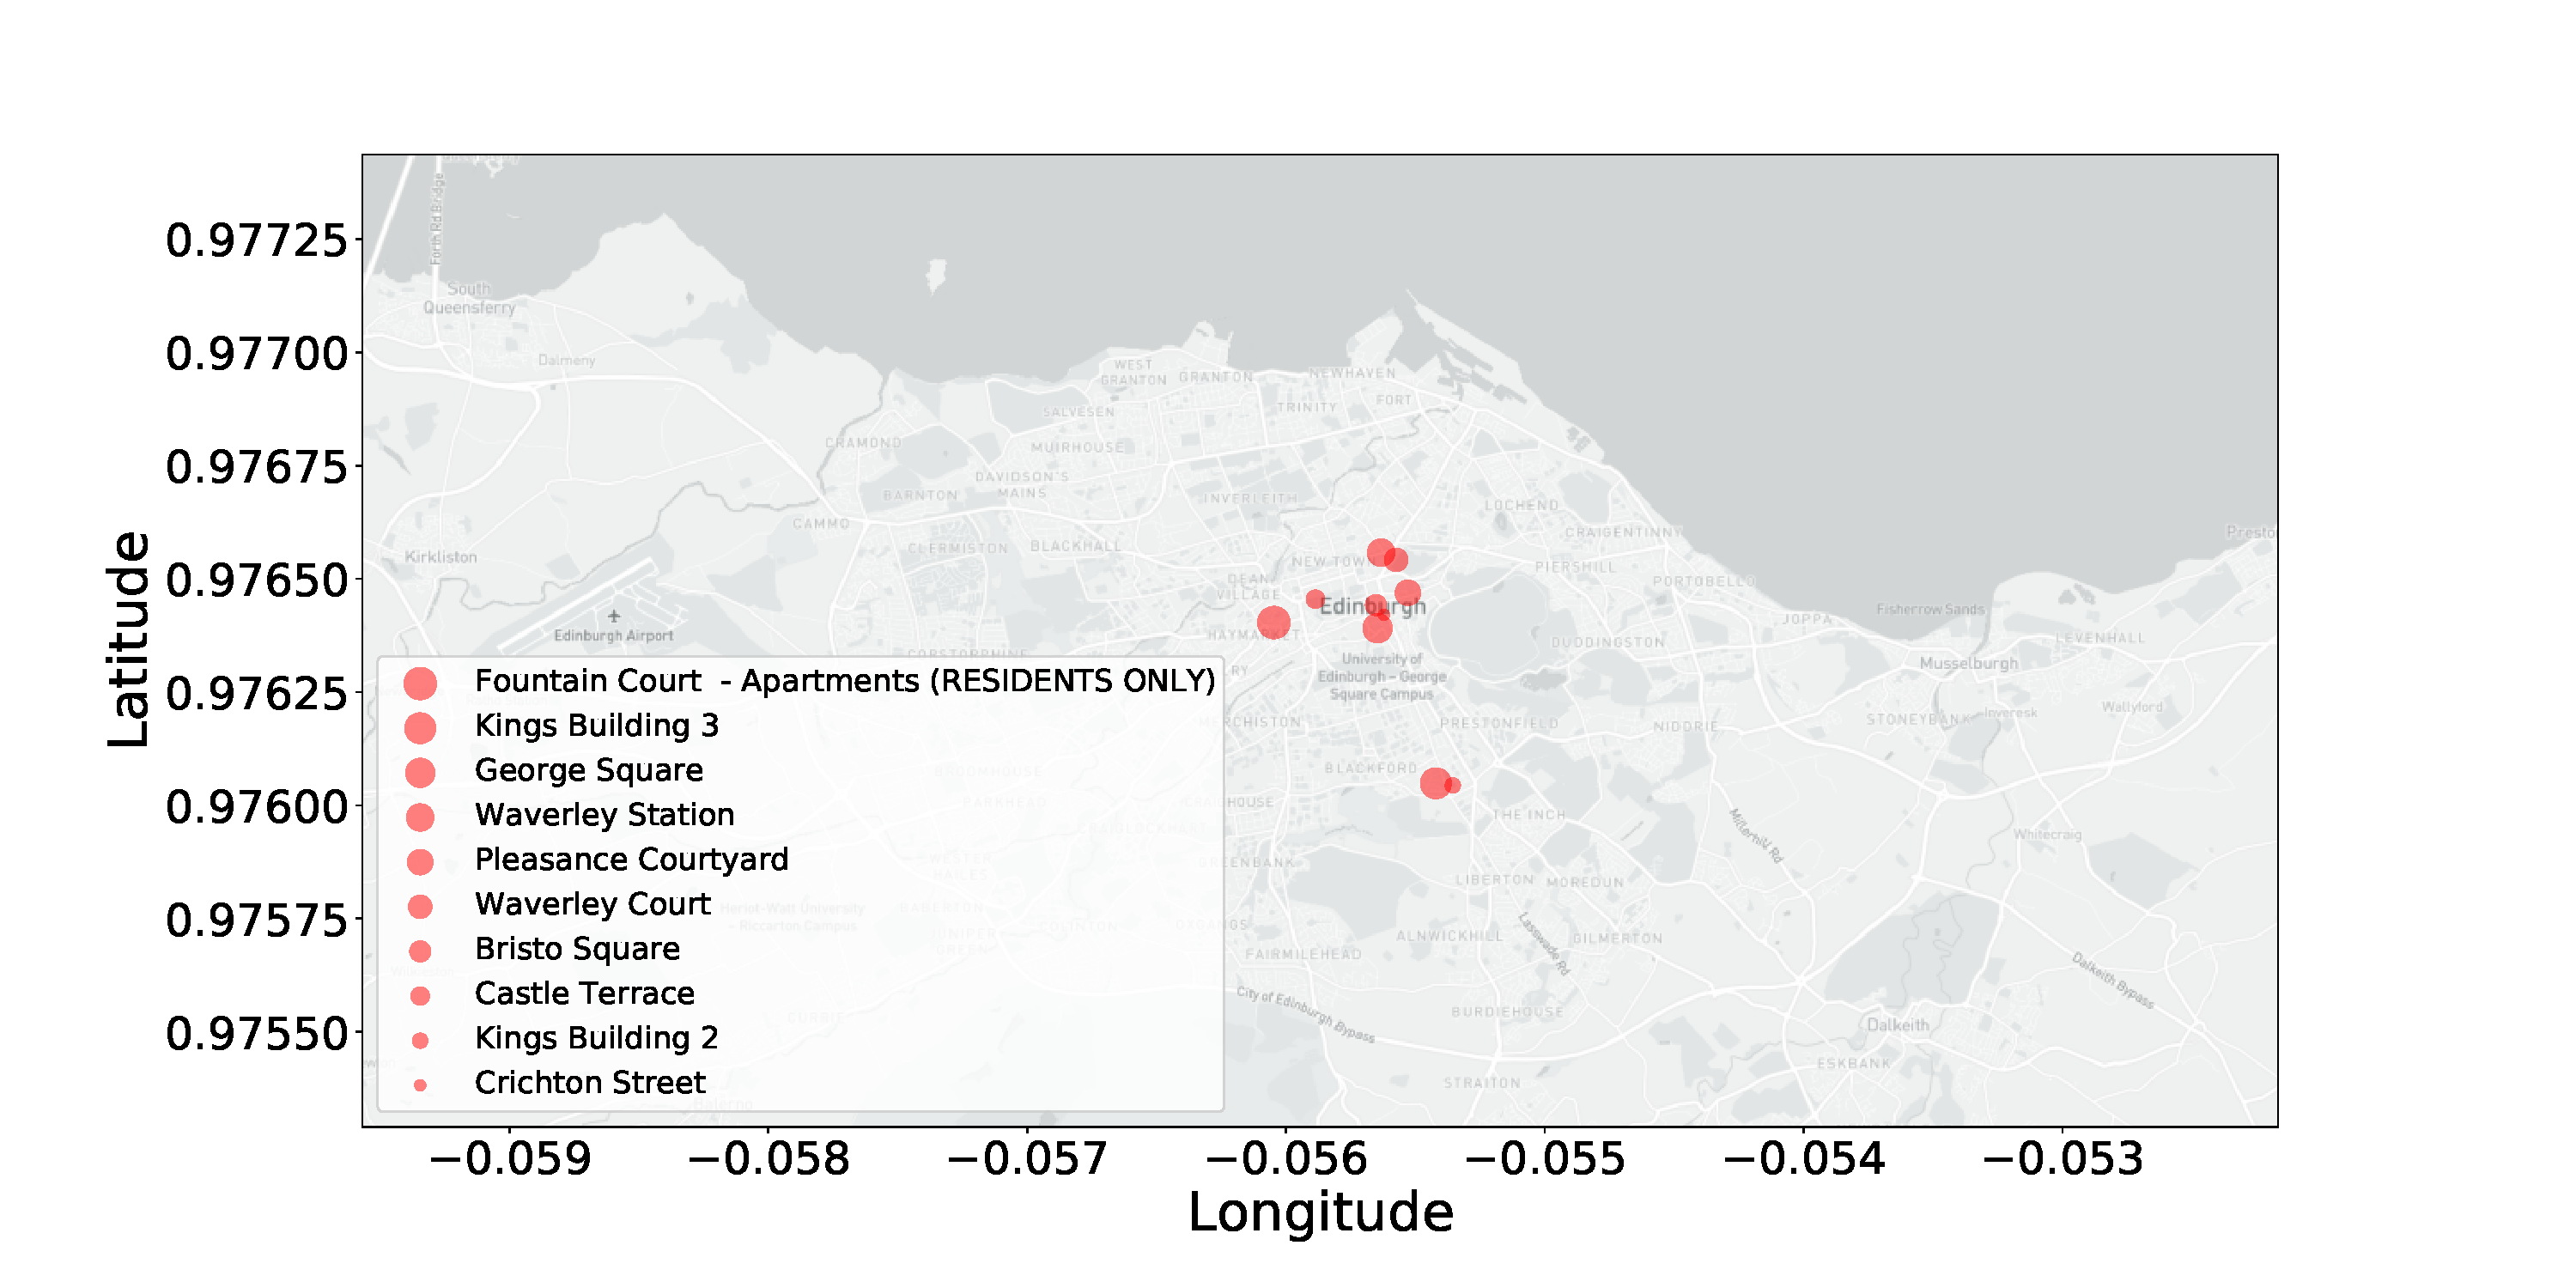
\includegraphics[scale=0.35]{datasets/stations_most_trips_percentage_drop.pdf}
    \vspace*{-1.2cm}
    \caption{Stations with greatest drop in popularity}
    \label{percentage_popularity}
\end{figure}
In Figure~\ref{percentage_popularity}, we can see that many of the student populated areas, such as the King's Buildings,  have seen a sizeable drop in number of trips due to the majority if not all lectures and the various other forms of teaching moving online for the academic year \cite{online}. Many stations in New Town have also suffered due to restrictions \cite{stores_princess}, with the stations around the Edinburgh Waverley railway station plummeting in numbers due to level three restrictions \cite{waverly}.

\section{Discussion and conclusions}
% Suggested 400 words.
\vspace{-5mm}
\paragraph{Summary of findings}
As we initially theorized, the COVID-19 pandemic had an impact on the usage of the bike sharing system in Edinburgh, more specifically restrictions due to lockdown affected, sometimes significantly, the  popularity of certain station and the reason for bike usage. However, contrary to our speculation, the number of trips increased. Reasons for this increase include: greater interest in cycling \cite{BBC_cycle}, avoidance of public transport due to health concerns and an increased number of bike docking stations. Many people started using bikes primarily for leisure, peaking in the evening which was not the case before the pandemic, with a bi-modal distribution representing usage of bikes (morning commute and leisure). Additionally, lockdown had an effect on the average duration of the bike trips as stated in out hypothesis test. 
\vspace{-4mm}
\paragraph{Evaluation of own work: strengths and limitations}
We were limited in the variety of data/data types available to us. Data about weather and average temperature would have allowed us to properly compare the impact of lockdowns on the number of trips taken as weather can also be a deciding factor if trips should take place or not. Information about usage of other forms of public transportation could have further reinforced our initial theories regarding the pandemic. However, we were able to isolate the effects of the pandemic from the effects of the weather on bike usage and then be able to use the information available to us on official government websites and news articles to back our claims.
\vspace{-4mm}
\paragraph{Comparison with any other related work}
Comparisons between cycling numbers in 2019 and 2020 in Scotland were made \cite{cycling_scot} with an increase of 68\% in April following the lockdown introduced in March of 2020 compared to the same time frame in 2019. Not only is cycling a popular activity in Scotland, but also one enjoyed in England \cite{england_cycle} with 16\% of the population cycling of England cycling per week during the pandemic. Cycling in Scotland had more then doubled according to the 'Discerning Cyclist' article with other modes of transportation falling by 95\%.
\vspace{-4mm}
\paragraph{Improvements and extensions}
We could extend our study to predict the purpose of a bike trip : leisure or work related, based on the start station. This can be done using k-means with which we can assign bike usage to a specific cluster. Instead of displaying the 'x' most popular start stations, we could use a heat-map to indicate the more popular areas for bike sharing and how that extends to other zones of the city. As mentioned above, data regarding other forms of transportation could have been obtained from other websites for comparisons between the different modes of transportation.

\bibliographystyle{unsrt}
\bibliography{fds-project}
\begin{thebibliography}{9}
\bibitem{who_wuhan} 
who.int, (2020). \textit{Archived: WHO Timeline-COVID-19}. Available online:
\texttt{https://www.who.int/news/item/27-04-2020-who-timeline---covid-19 [Accessed 05 Apr. 2021]}.
\bibitem{tayside}
Mitchell, H. (2020). \textit{Coronavirus in Tayside: first confirmed case of deadly illness caused by COVID-19 in Scotland}. [online] edinburghlive. Available online: \texttt{https://www.edinburghlive.co.uk/news/uk-world-news/coronavirus-tayside-
first-confirmed-case-17843361} [Accessed 03 Apr. 2021].
\bibitem{timeline}
spice-spotlight.scot, (2021). \textit{Timeline of Coronavirus (COVID-19) in Scotland}. [online] Available online: \texttt{https://spice-spotlight.scot/2021/03/19/timeline-of-coronavirus-covid-
19-in-scotland/} [Accessed 30 Mar. 2021].
\bibitem{london_bombing}
Fasolo, Barbara; Ni, Zhifang; and Phillips, Lawrence D., A Study Of The Impact Of The July Bombings On Londoners’ Travel Behaviour" (2008). Non-published Research Reports. City: London. Paper 17. [Accessed 31 Mar. 2021]
\bibitem{greece_covid}
Nikiforiadis, A.; Ayfantopoulou, G.; and Stamelou ,A. \textit{Assessing the Impact of COVID-19 on Bike-SharingUsage: The Case of Thessaloniki, Greece} (2020). Centre for Research and Technology Hellas. City: Thermi. 12 Pages. [Accessed 29 Mar. 2021] 
\bibitem{texas_covid}
Jobe , J.; P.Griffin ,G. \textit{Bike share responses to COVID-19} (2021). Transportation Research Interdisciplinary Perspectives. City: San Antonio. 7 Pages.[Accessed 04 Apr. 2021]
\bibitem{hire_scheme}
The Edinburgh Reporter.
\textit{100,000 trips on Just Eat bikes in a year} (2019) Available online:
\texttt{https://theedinburghreporter.co.uk/2019/09/100000-trips-on-just-eat-bikes-
in-a-year/} [Accessed 07 Apr. 2021].
\bibitem{average_temp}
worldweatheronline.com, (2020). \textit{Edinburgh Monthly Climate Averages}. Available online:
\texttt{https://www.worldweatheronline.com/edinburgh-weather-averages/city-of-
edinburgh/gb.aspx} [Accessed 06 Apr. 2021].
\bibitem{snow_storm}
Claire Galloway (2021). \textit{Storm Darcy hits LIVE as weather warning upgraded to amber for Edinburgh}. Available online: \texttt{https://www.edinburghlive.co.uk/news/edinburgh-news/edinburgh-weather-live-
capital-blasted-19798565} [Accessed 06 Apr. 2021]
%https://www.holiday-weather.com/edinburgh/averages/
\bibitem{stores_princess}
Pope, I. (2020). \textit{Just five shops open on Princes Street amid coronavirus lockdown}. Edinburgh News. Available online: \texttt{https://www.edinburghnews.scotsman.com/health/coronavirus/just-five-shops
-open-princes-street-amid-coronavirus-lockdown-2518975} [Accessed 01 Apr. 2021]
\bibitem{establishments}
Smith, J. (2020). \textit{Coronavirus: all the Edinburgh pubs that have closed so far as other businesses call for help}. edinburghlive. Available online: \texttt{https://www.edinburghlive.co.uk/news/edinburgh-news/coronavirus-edinburgh-
pubs-closed-far-17944618} [Accessed 03 Apr. 2021]
\bibitem{online}
ed.ac.uk, (2021). Information about Semester 2. [online] Available online: \texttt{https://www.ed.ac.uk/news/covid-19/current-students/semester-2} [Accessed 30 Mar. 2021].
\bibitem{waverly}
Morrow, D. (2020). \textit{Eerie snap shows Edinburgh Waverley Station looking like a ghost town}. edinburghlive, [online]. Available online: \texttt{https://www.edinburghlive.co.uk/news/edinburgh-news/eerie-snap-shows-
edinburgh-waverley-19492776} [Accessed 05 Apr. 2021].
\bibitem{BBC_cycle}
Bernhard, A. (2020). \textit{The great bicycle boom of 2020}. [online] Available online: \texttt{https://www.bbc.com/future/bespoke/made-on-earth/the-great-bicycle-boom-of-
2020.html} [Accessed 06 Apr. 2021] 
\bibitem{cycling_scot}
cycling.scot, (2020). \textit{Six-month stats see cycling up 43\% in Scotland}. [online] Available at: \texttt{https://www.cycling.scot/news-and-blog/article/six-month-stats-see-cycling-up
-43-in-scotland} [Accessed 07 Apr. 2021].
\bibitem{england_cycle}
Chandler, M. (2020). \textit{8.9 Million People Cycling in England During the COVID-19 Pandemic}. [online] Available online: \texttt{https://discerningcyclist.com/cycling-covid-19-pandemic-statistics-uk/} [Accessed 09 Apr. 2021]
\end{thebibliography}
\end{document}